\documentclass[12pt,a4paper]{article}
\usepackage[utf8]{vietnam}
\usepackage[left=2.5cm, right=2cm,top=2cm, bottom=2cm]{geometry}
\usepackage{amsmath,amsfonts,amssymb}
\usepackage{tikz}
%\usetikzlibrary{}

\begin{document}
	\noindent Vẽ lại các hình sau bằng TikZ.\\[5mm]
	%hình 1
	\begin{center}
		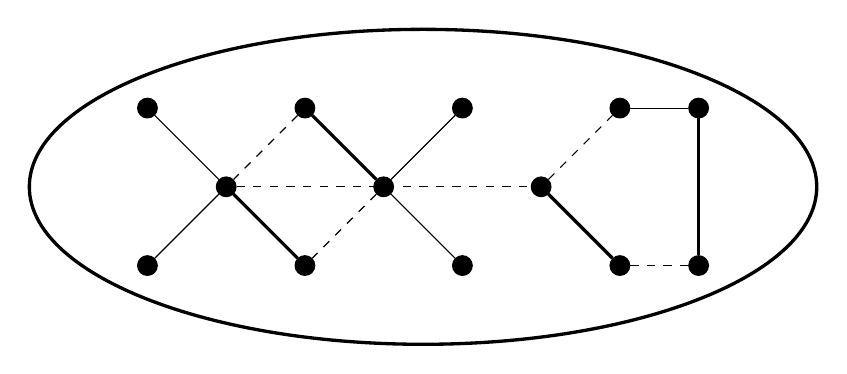
\begin{tikzpicture}[mystyle/.style={circle, draw=black, fill=black, inner sep=0pt, minimum size=2.5mm}]
			\node (1) at (0,0) [mystyle] {};
			\node (2) at (2,0) [mystyle] {};
			\node (3) at (4,0) [mystyle] {};
			\node (4) at (6,0) [mystyle] {};
			\node (5) at (7,0) [mystyle] {};
			\node (6) at (0,2) [mystyle] {};
			\node (7) at (2,2) [mystyle] {};
			\node (8) at (4,2) [mystyle] {};
			\node (9) at (6,2) [mystyle] {};
			\node (10) at (7,2) [mystyle] {};
			\node (11) at (1,1) [mystyle] {};
			\node (12) at (3,1) [mystyle] {};
			\node (13) at (5,1) [mystyle] {};
			
			\draw (1)--(11);
			\draw (11)--(6);
			\draw[dashed] (7)--(11);
			\draw[very thick] (11)--(2);
			\draw[dashed] (11)--(13);
			\draw[very thick] (7)--(12);
			\draw[dashed] (12)--(2);
			\draw (12)--(3);
			\draw (12)--(8);
			\draw[very thick] (13)--(4);
			\draw[very thick] (5)--(10);
			\draw (9)--(10);
			\draw[dashed] (13)--(9);
			\draw[dashed] (4)--(5);
			\draw[very thick] (3.5,1) circle (5 and 2);
		\end{tikzpicture}
	\end{center}\,\\[5mm]
	
	%hình 2
	\begin{center}
		\begin{tikzpicture}
			\draw[thick] (0,0)--(10,0);
			\draw[thick] (10,3)--(10,-3) node[below left] at (10,0) {$O$};
			\draw[thick] (5,3)--(5,1.1) (5,1)--(5,-1) (5,-1.1)--(5,-3) node[right] at (5,1) {$S_1$} node[right] at (5,-1) {$S_2$};
			\draw[thick,|<->|] (10.5,0)--(10.5,1) node[right] at (10.5,.5) {$5mm$};
			\draw[thick,|<->|] (4.5,-1)--(4.5,1) node[left] at (4.5,.5) {$10mm$};
			\draw[thick,|<->|] (5,-2)--(10,-2) node[above] at (7.5,-2) {$2m$};
			\draw[thick,|<->|] (5,-2)--(1.5,-2) node[above] at (3.25,-2) {$1m$};
			\draw[thick,|<->|] (1.5,0)--(1.5,0.3) node[left] at (1.5,0.2) {$1mm$};
			\node[label=above right: $P$] at (10,1) {};
			\node[label=above right: $S$] at (1.5,0.3) {};
		\end{tikzpicture}
	\end{center}\,\\[5mm]
	
	%hình 3
	\begin{center}
		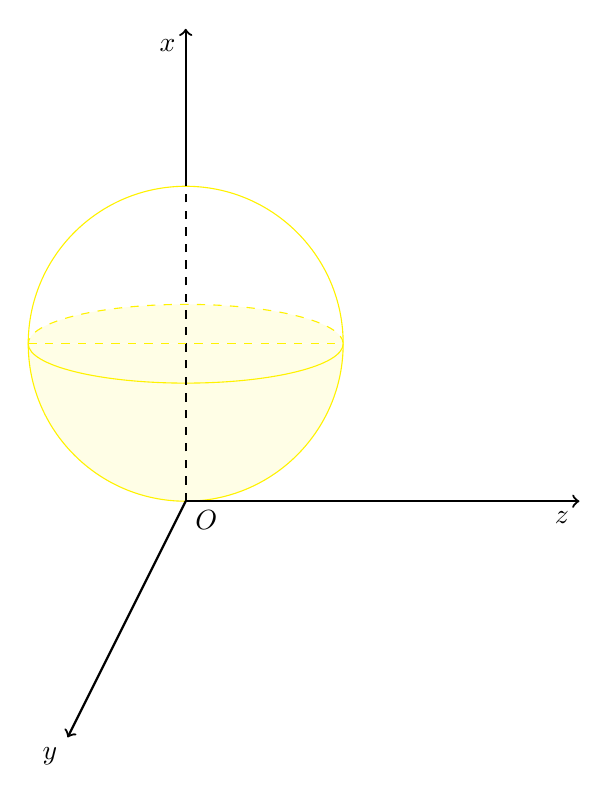
\begin{tikzpicture}
			\draw[draw=yellow, fill=yellow!10] (-2,2) arc (180:360:2);
			\draw[draw=yellow] (2,2) arc (0:180:2);
			\draw[draw=yellow, fill=yellow!10, dashed] (2,2) arc (0:180:2 and 0.5);
			\draw[draw=yellow] (-2,2) arc (180:360:2 and 0.5);
			
			\draw[thick,->](0,4)--(0,6)node[anchor=north east]{$x$};
			\draw[thick,->](0,0)--(-1.5,-3)node[anchor=north east]{$y$};
			\draw[thick,->](0,0)--(5,0)node[anchor=north east]{$z$};
			\draw [thick,dashed] (0,0)--(0,4);
			\draw[ draw= yellow, dashed] (-2,2) -- (2,2);
			
			\node [below right] at (0,0) {$O$};
		\end{tikzpicture}
	\end{center}
	\pagebreak
	
	%hình 4
	\begin{center}
		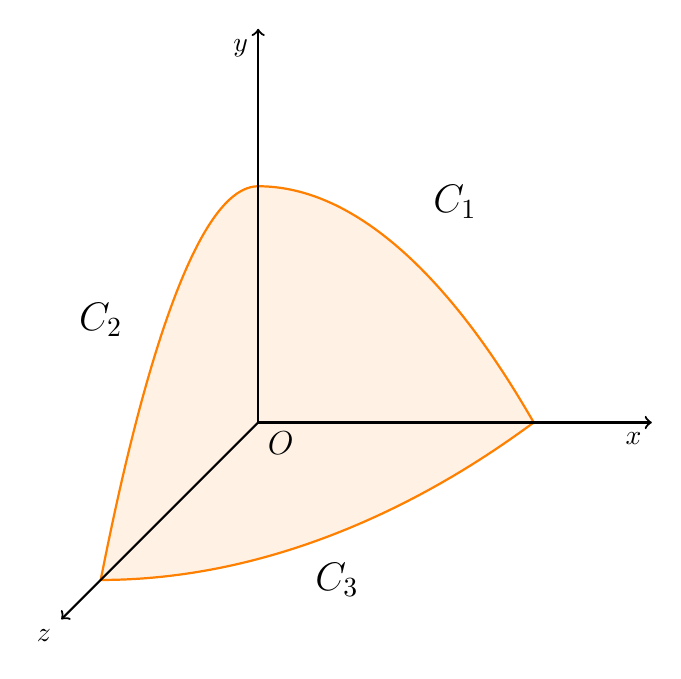
\begin{tikzpicture}
			\draw[orange!10, fill=orange!10] (0,3)--(-2,-2)--(3.5,0)--cycle;
			\draw[thick, orange, fill=orange!10] (0,3) parabola (-2,-2);
			\draw[thick, orange, fill=orange!10] (-2,-2) parabola (3.5,0);
			\draw[thick, orange, fill=orange!10] (0,3) parabola (3.5,0);
			\draw[thick,->](0,0)--(5,0)node[anchor=north east]{$x$};
			\draw[thick,->](0,0)--(0,5)node[anchor=north east]{$y$};
			\draw[thick,->](0,0)--(-2.5,-2.5)node[anchor=north east]{$z$};
			\node[below right] at(0,0) {\large$O$};
			\node at (-2,1.3){\Large\bfseries$C_2$};
			\node at (2.5,2.8){\Large\bfseries$C_1$};
			\node at (1,-2){\Large\bfseries$C_3$};
		\end{tikzpicture}
	\end{center}\,\\[5mm]
	
	%hình 5
	\begin{center}
		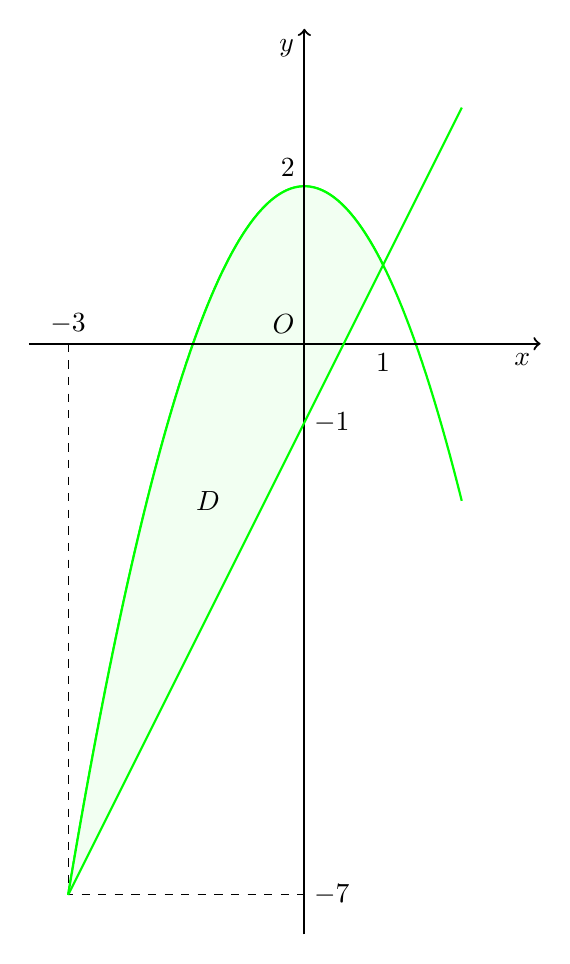
\begin{tikzpicture}
			\draw[thick,green,domain=-3:2,samples=100] plot ({\x},{2-(\x)^2});
			\draw[thick,green,fill=green!5,domain=-3:1,samples=100] plot ({\x},{2-(\x)^2});
			
			\draw[thick, ->](0,-7.5)--(0,4) node [anchor= north east]{$y$};
			\draw[thick, ->](-3.5,0)--(3,0) node [anchor= north east]{$x$};
			\draw[dashed] (-3,0)--(-3,-7)--(0,-7);
			
			\draw[thick,green,domain=-3:2,samples=50] plot ({\x},{2*(\x)-1});
			
			\node [above] at (-3,0) {$-3$};
			\node [above left] at (0,0) {$O$};
			\node [below] at (1,0) {$1$};
			\node [above left] at (0,2) {$2$};
			\node [right] at (0,-1) {$-1$};
			\node [right] at (0,-7) {$-7$};
			\node [right] at (-1.5,-2) {$D$};
		\end{tikzpicture}
	\end{center}
	
	
	
\end{document}